% Modified based on Xiaoming Sun's template

% Modified based on Xiaoming Sun's template

\documentclass{article}
\usepackage{amsmath,amsfonts,amsthm,amssymb}
\usepackage{indentfirst}
\usepackage{setspace}
\usepackage{fancyhdr}
\usepackage{lastpage}
\usepackage{extramarks}
\usepackage{chngpage}
\usepackage{soul,color}
\usepackage{graphicx,float,wrapfig}
\usepackage{ifpdf}
%\usepackage{CJKspace}
\usepackage{verbatim}
%\usepackage{ctex}
\usepackage{algorithm}
\usepackage{algorithmicx}
\usepackage{algpseudocode}
\usepackage{url}

%\usepackage{natbib}

\usepackage[colorlinks, citecolor=blue]{hyperref}


% In case you need to adjust margins:
% \topmargin=-0.45in      %
% \evensidemargin=0in     %
% \oddsidemargin=0in      %
% \textwidth=6.5in        %
% \textheight=9.0in       %
% \headsep=0.25in         %

% Setup the header and footer
% \pagestyle{fancy}                                                       %
% \chead{\Title}  %
% \rhead{\firstxmark}                                                     %
% \lfoot{\lastxmark}                                                      %
% \cfoot{}                                                                %
% \rfoot{Page\ \thepage\ of\ \protect\pageref{LastPage}}                          %
% \renewcommand\headrulewidth{0.4pt}                                      %
% \renewcommand\footrulewidth{0.4pt}                                      %

% �����Զ���һЩ����
\newcommand{\Answer}{\ \\\textbf{Answer:} }
\newcommand{\Acknowledgement}[1]{\ \\{\bf Acknowledgement:} #1}
\newcommand{\Reference}[1]{\ \\{\bf Reference:} #1}
\newtheorem{theorem}{Theorem}

\newcommand\numberthis{\addtocounter{equation}{1}\tag{\theequation}}


    %%%%%%%%%%%%%%%%%%%%%%%%%%%%%%%%%%%%%%%%%%%%%%%%%%%%%%%%%%%%%


    %%%%%%%%%%%%%%%%%%%%%%%%%%%%%%%%%%%%%%%%%%%%%%%%%%%%%%%%%%%%%
    % ���ⲿ��
    \title{\textmd{\bf Artificial Intelligence Project -- Progress}}
    \date{}
    \author{Yiheng Lin, Zhihao Jiang}
    %%%%%%%%%%%%%%%%%%%%%%%%%%%%%%%%%%%%%%%%%%%%%%%%%%%%%%%%%%%%%

    \begin{document}
    \begin{spacing}{1.1}
    \maketitle %\thispagestyle{empty}

    %%%%%%%%%%%%%%%%%%%%%%%%%%%%%%%%%%%%%%%%%%%%%%%%%%%%%%%%%%%%%
    % Begin edit from here
    \section{Introduction}
    It is widely accepted that h-DQN (Hierarchy Deep Q-Learning) is developed to tackle the efficiency problem of $\epsilon -$greedy Q-Learning when the reward is sparse. However, after we study the problem setting and reimplement the method proposed in \cite{AI-16}, we find another big advantage of h-DQN over traditional Q-Learning and DQN (Deep Q-Learning) \cite{AI-15} is that h-DQN can potentially discover the hidden state which is not observable by the agent but is crucial for receiving reward. To make our idea more clear, let us consider the following game (proposed in (1)):
    \subsection{Game Setting}
    The state set is $S = \{1, 2, \cdots, 6\}$ and the action set is $A = \{1, 2\}$. The agent start at state 2 and state 1 is the terminal state. At state i, if the agent takes action 1, it will go to state $i-1$ with probability 1; if the agent takes action 2, it will go to state $i+1$ with probability 0.5;otherwise, it will go to state $i-1$. The reward is received at state 1: if the agent has been to state 6, it will receive reward 1; otherwise, it will receive reward $0.01$.

    \begin{center}
        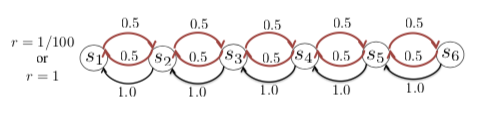
\includegraphics[width = 0.5\textwidth]{game.png}
    \end{center}

    The authors of \cite{AI-16} claim that traditional Q-Learning cannot learn to take action 2 in order to move towards state 6 even after a long period of training (200 epochs) and converges to a sub-optimal policy. Our experiment shows the same result.

    Actually, despite the length of the path of the optimal policy and the probability setting on state transition, we think the major difficulty in this game is the hidden state of whether the agent has reached state 6. At state i $(2\leq i\leq 5)$, when state 6 has not been reached, the agent should take action 2 in order to reach 6, which means $Q(i, 2) > Q(i, 1)$; when state 6 has already been reached, the agent should take action 1, which means $Q(i, 2) < Q(i, 1)$ (Although keep taking action 2 is a possible optimal policy, we think it is almost impossible for the agent to keep taking action 2 after state 6 has been reached, since it cannot see the difference in the final reward.). In traditional Q-Learning and DQN, QValue function should converge as learning proceed, thus it is difficult for them to learn the optimal policy even unlimited time is given.

    However, if the hidden state is given to tell the agent whether it has reached state 6, (for example, 0 represents it has not visited state 6, 1 represents it has visited state 6) then the problem is converted to a MDP of 12 states. Then at state i, the agent can separately learn $Q((i, 0), 2) > Q((i, 0), 1)$ and $Q((i, 1), 2) < Q((i, 1), 1)$. We think this will make the problem much easier for traditional Q-Learning. We will do more experiments to verify this claim. The subgoal in \cite{AI-16} operates similarly, the meta-controller should first set the subgoal to state 6 and then set the subgoal to state 1 after state 6 is visited.

    In the real world, it is very common that the final outcome of a game actually depends on some hidden state that the agent can not observe. So this problem, although not very complicated, can provide important insight to solve real problems with hidden states. h-DQN algorithm provides an potentially efficient way to let the agent, which combines controller and meta-controller, learn about the important hidden states.
    \subsection{H-DQN Algorithm}
    We carefully studied algorithm 1 proposed by \cite{AI-16} (please find the pseudocode in appendix 1) and reimplement this algorithm on the game setting described in the last section based on \cite{github}. We can see salient improvement compared with traditional Q-Learning method, although the performance is worse than the authors of \cite{AI-16} claimed. After supervising the training process, we think there are some potential improvements we can do to judge the effectiveness of h-DQN algorithm.

    Roughly speaking, the h-DQN algorithm works as following: the meta-controller (higher hierarchy) sets a subgoal state for controller (lower hierarchy); then the controller tries to move to the subgoal state since it will get an intrinsic reward of 1 if it succeed in reaching the subgoal and no intrinsic reward if it fails to reach the subgoal; the meta-controller collects the extrinsic reward gotten by the agent for different (state, subgoal) pairs and decide which state should be the next subgoal.

    As for the performance metric, the authors of \cite{AI-16} uses the number of visits to each state during 1000 runs to judge the agents tendency of taking action 2. However, a lot of visits to state 6 is resulted by keep taking action 2 after arriving at state 6. So the agents can visit state 6 multiple times in one run. Thus we think we should instead evaluate the probability the agent arrives at state 6 in each run.
    \begin{center}
        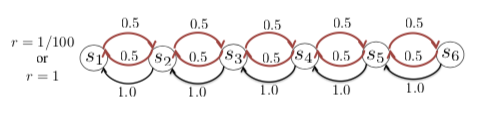
\includegraphics[width = 0.5\textwidth]{game.png}
    \end{center}
    \begin{theorem}
    If the optimal policy is chosen (i.e. keep taking action 2 until state 6 is arrived), the probability of arriving at state 6 is $\frac{1}{5}$.
    \end{theorem}
    \begin{proof}
        Since we only consider whether state 6 can be reached, in the proof, we can let state 6 be a terminal state. Let $x_i$ be the probability of arriving state 6 from state i $(1\leq i \leq 6)$, then we have $x_1 = 0, x_6 = 1$, and
        \begin{equation}
            x_i = 0.5x_{i-1} + 0.5x_{i+1}, (2\leq i \leq 5)
        \end{equation}
        Solving the equations and we can get $x_2 = \frac{1}{5}$.

        Notice that if we adopt $\epsilon -$greedy policy, equation (1) will become
        \begin{equation}
            x_i = \frac{1 + \epsilon}{2}x_{i-1} + \frac{1 - \epsilon}{2}x_{i+1}, (2\leq i \leq 5)
        \end{equation}
        When $\epsilon = 0.1$, we can get $x_2 = 0.128645$.
    \end{proof}
    This theorem shows that the probability the agent arrives at state 6 in each run should be near $0.128$ if the policy is near optimal when $\epsilon = 0.1$.

    Another observation is that when the subgoal is set to state 2, the controller (lower hierarchy) opts to choose action 2 frequently even when it is at state 3, 4, 5, and consequently arrives at state 6 with high probability. This encourages the meta-controller (higher hierarchy) to set the subgoal to state 2 since the meta-controller will see setting subgoal 2 often results in a good extrinsic reward. This result is unexpected, and not robust, since the intrinsic reward is given to the controller only when it arrives at state 2, we can never promise that the agent will always try to go to state 6 before arrives at state 2 during long period of learning. We think this phenomena occurs because the experience provided to the meta-controller is highly unstable during the training. The controller may has learned a suboptimal policy to reach its subgoal, but this suboptimal policy results in a good extrinsic reward, which is favored by the meta-controller. When we see good average rewards, the model may have not been converged. And maybe at some time the controller may find a new way to reach its subgoal, then the average reward collapses dramatically, as we see when running experiment. So we think in the further experiments, we should measure the meta-controller's ability of setting reasonable subgoals; and the actions the controller takes to achieve them.

    \section{Our Attempt}

    \subsection{Intuition}

    Draw subgoal randomly is a new method to set subgoal. Because it urge the agent to explore new states rather than stay in local optimal states. In the game we just mentioned, the agent tends to go left if using $\epsilon-$greedy because of the transport probability. However, in hierarchical model, the agent tends to the subgoal. If we draw subgoal randomly, the agent will explore efficiently.

    Based on this method, we attempt to modify the method a little bit.

    To explore new states, besides draw subgoal randomly, we can also draw the state which we have least information about.

    There are several ways to implement this idea such as drawing the farthest state away the current state, drawing randomly from states which are not arrived before. Another idea is, define the distance between two states in some way, and draw a subgoal such that the subgoal is "close" to lots of states which are not arrived before. We will attempt to implement this idea in models which is more complicate than the model we just mentioned.

    \subsection{Progress}

    Although the idea is not implemented in general model, it is easy to implement the idea in the simple model we mentioned. That is, set the farthest state as the subgoal.

    In detail, the agent start at state 2. We always set subgoal as the farthest state (state 6 initially). The subgoal is not changed until the agent arrive the state. Once the agent arrive the subgoal, we reset the subgoal as the farthest state away the current state. For the lower controller, the closer to the subgoal, the larger the reward is, so the agent tends to the subgoal.

    The chart below is the experiment result. The $x-$axis is time, and the $y-$axis is grade. The blue, red, yellow lines is corresponding to the method $\epsilon-$greedy, random subgoal, farthest subgoal respectively.

    
\includegraphics[width=90mm]{1.png}

    We can see the yellow line raises abruptly when the process is 60\% done. Maybe this is because the parameter should be adjusted, or there are some other reasons.

    \subsection{Plan of following work}

    As what we talking, some problems still remains. We will attempt to deal with them, such as
    \begin{itemize}
        \item Why the yellow line raises abruptly
        \item How to implement our idea in more general model
        \item Is this idea useful to DQN
    \end{itemize}

    Besides, maybe our method is targeted at this special model, we should assess the generalization of our method and modify the method if needed.


    \section*{Appendix}

    \subsection*{The algorithm in the paper}
    \begin{center}
        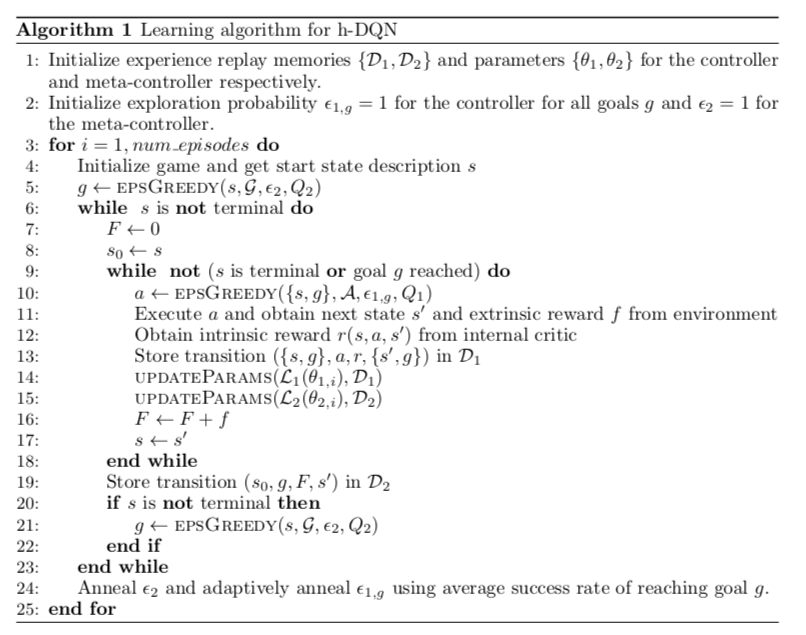
\includegraphics[width = \textwidth]{pseudo.png}
    \end{center}

    \subsection*{Our codes}
    \url{https://github.com/faebdc/AI-Project}
    (There is README for details)

    \bibliographystyle{plain}
    \bibliography{refx}

    \Acknowledgement{}

    % End edit to here
    %%%%%%%%%%%%%%%%%%%%%%%%%%%%%%%%%%%%%%%%%%%%%%%%%%%%%%%%%%%%%

    \end{spacing}
    \end{document}

    %%%%%%%%%%%%%%%%%%%%%%%%%%%%%%%%%%%%%%%%%%%%%%%%%%%%%%%%%%%%%

